\chapter{Research Design}
\par{This chapter outlines the research design employed to in the study. The aim is to investigate and reveal the most optimal research methodology and paradigm that encourage the success of the case study. The methodology encompasses Design Science Research (DSR) within the positivist paradigm, emphasising the creation and evaluation of innovative artefacts to address specific challenges. Data collection will primarily involve monitoring a case study, supplemented by interviews with experts, with analysis conducted through quantitative methods.}
\par{The following chapter will explore and pinpoint areas of relevance to the study within the domain of research design. The chapter begins by examining various research methodologies relevant to the field and discussing the chosen methodology to be used in greater depth, addressing the relevant literature and the effect these findings will have on the research project at hand. The same exploration is then done on research paradigms and which will be most suitable and fitting for the current study, concurrently addressing the affect the choice will have on the research project. The chapter then continues to delve into methodologies for determining the success of completion of the artefact and makes use of that information to determine what data collection will be done so that a quantitative conclusion can be made at the end of the study. The rest of the chapter defines how the research is designed and how it will be conducted, as well as how ethical clearance is acquired and what ethical implications the project could have.}


\section{Exploring Research Methods using the Research Onion}
\par{When doing research, the research onion created by \cite{saunders2009research} is frequently used as a design guide. A growing number of researchers from different disciplines are increasingly embracing the research onion model as a basis for their study design, despite its original primary use in business research. The layers of the research onion represent several aspects of formulating a research strategy, the outer layers are more theoretical and the interior levels more practical \citep{saunders2009research}. The figure below shows the research onion that was outlined by \cite{saunders2009research}.}
\begin{figure}[h!]
    \centering
    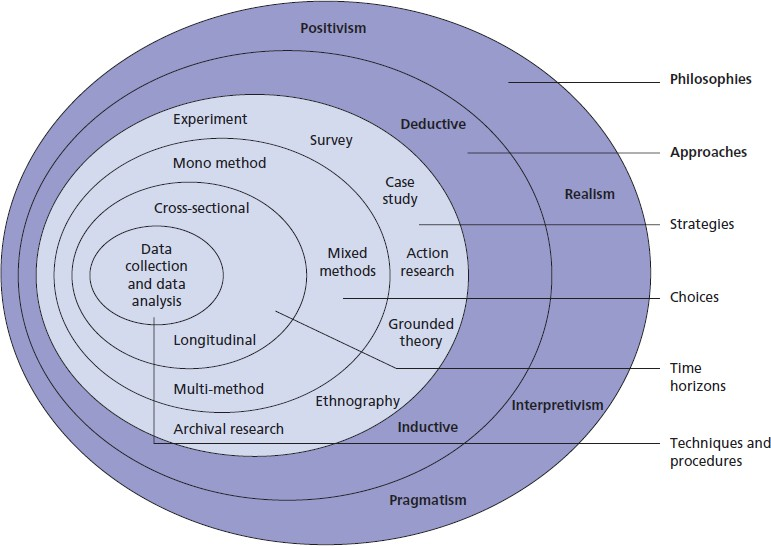
\includegraphics[width=1\linewidth]{img/Saunders research onion.jpg}
    \caption{The Saunders Research Onion}
    \label{fig:enter-label}
\end{figure}
\par{Since IS is a field of study that integrates both the natural and social sciences, employing the research onion as proposed by \cite{saunders2009research} in and of itself requires some adjustments as it has not yet taken into account all the techniques and strategies used in the field of IS. Therefore, \cite{mardiana2020modifying} proposed a modified version of the research onion that is more catered towards the field of information science research. The modified version of the research onion can be seen in the figure below.}
\clearpage
\begin{figure}[h!]
    \centering
    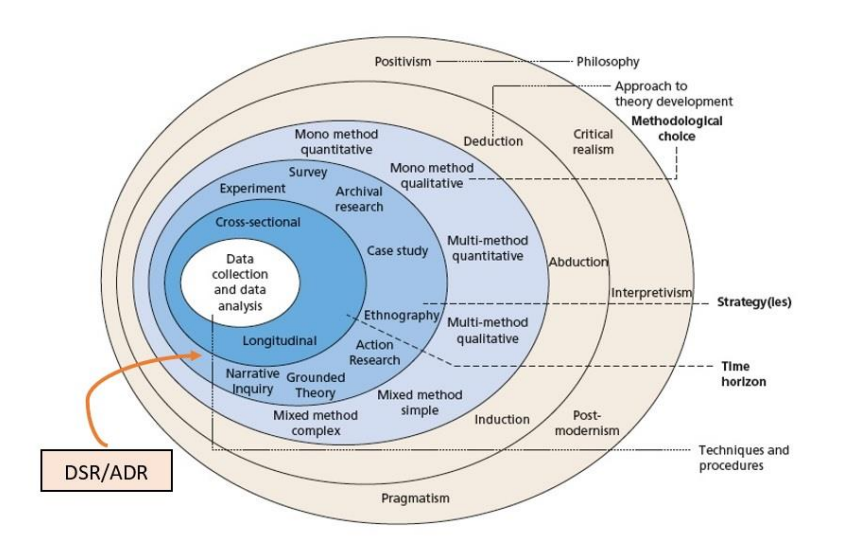
\includegraphics[width=1\linewidth]{img/Modified research Onion.png}
    \caption{The Modified Research Onion}
    \label{fig:enter-label}
\end{figure}
\par{As it is some what difficult to understand the implications of the modified research onion, \cite{mardiana2020modifying} also provides the following table showing how research design can be constructed by making use of the modified research onion.}
\begin{table}[h!]
\centering
\small 
\begin{adjustbox}{max width=\textwidth}
\begin{tabular}{|p{2.2cm}|p{2.2cm}|p{2.2cm}|p{2.2cm}|p{2.5cm}|p{2.5cm}|}
\hline
\textbf{Philosophy} & \textbf{Approach} & \textbf{Methods} & \textbf{Strategy} & \textbf{Time horizon} & \textbf{Data collected} \\
\hline
Positivism & Deductive & Quantitative & Experiment & Cross-sectional Longitudinal & Numerical \\
\hline
Positivism & Deductive & Quantitative & Survey & Cross-sectional Longitudinal & Numerical \\
\hline
Interpretivism & Inductive & Qualitative & Archival research & Cross-sectional & Non-Numerical \\
\hline
Interpretivism & Inductive & Qualitative & Case study & Cross-sectional & Non-Numerical \\
\hline
Interpretivism & Inductive & Qualitative & Ethnography & Cross-sectional & Non-Numerical \\
\hline
Interpretivism & Inductive & Qualitative & Action Research & Cross-sectional & Non-Numerical \\
\hline
Positivism Interpretivism Pragmatism & Abductive Deductive & Quantitative Qualitative & Design research & Cross-sectional Longitudinal & Numerical Non-Numerical \\
\hline
Interpretivism & Inductive & Qualitative & Grounded theory & Cross-sectional & Non-Numerical \\
\hline
Interpretivism & Inductive & Qualitative & Narrative inquiry & Cross-sectional & Non-Numerical \\
\hline
\end{tabular}
\end{adjustbox}
\caption{The possible research design composition in IS research}
\end{table}
\par{The research onion and its recommendations will be used to construct the research design that will be employed by this research project, as it provide guidelines for which options of the various components of research align with one another and are well suited. Each component of research, namely philosophy, approach, methods, strategy, time horizon, and date collected, will be further researched and investigated throughout the rest of this chapter in order to define the complete design of the research project.}


\section{Research Philosophy}
\par{A research philosophy explains the study's methods and the type of knowledge that was produced, as well as the researcher's viewpoint on the relationship between knowledge and development. The subsections that follow outline the various philosophies that form part of the modified research onion created by\cite{mardiana2020modifying}. Each philosophy will be studied independently in order to determine the viability of the outlook in the context of the research being conducted.}
\subsection{Positivism}
\par{Philosophers Descartes and Locke served as major influences during the 17th and 18th century Enlightenment, which is when positivism first emerged \citep{park2020positivism}. Over time, logical positivism also began to emerge. The idea that there is a universal, temporal truth that all disciplines must adhere to is greatly influenced by logical positivism, which holds that although scientific laws frequently emerge through the use of intuition, this does not entail that the laws can be subjectively justified \citep{luczak2013beyond}. Moreover, logical positivism's theory of truth consists of providing a solution to the following query: "For every given statement p, what are the conditions under which p (is true) and what are the conditions under which not-p?". Therefore, "a priori" (such as mathematical axioms) and "empirical" propositions—both of which require rigorous and open validation—are central to the logic of positivism \citep{luczak2013beyond}. Positivism, which is frequently connected to experiments and quantitative research, is seen as an evolution or kind of empiricism \citep{potrac2014interpretivism} Essentially, positivism comes down to the following: reliable findings can only come from occurrences that can be observed, and the researcher has no control over the findings of the investigation. Therefore, the researcher has no control over the study's outcomes.}
\par{The philosophical position of positivism is based on natural scientists' use of observed reality in society to generate generalisations. Positive thinking emphasises the value of information in general and places a stronger emphasis on considering facts and pure data free from human bias or interpretation \citep{saunders2009research}. If a researcher were to embrace an extreme positivist standpoint, several consequences would ensue \citep{alharahsheh2020review}:
\begin{itemize}
    \item The researcher would regard organisations or other related social entities as tangible entities, akin to physical objects and natural phenomena.
    \item Epistemologically, the research focus would prioritise the identification of observable and quantifiable facts or patterns. Moreover, the phenomena subjected to observation and measurement should contribute to the establishment of credibility and significance in the collected data.
    \item The researcher's objective would be to uncover causal relationships among the gathered data, facilitating the formulation of law-like generalisations akin to those formulated by scientists. Additionally, the researcher would utilise and incorporate fundamental universal principles and laws to justify and elucidate the behaviour or events studied within organizations.
\end{itemize}}
\par{Based on the requirements of the research project and its nature, the positivist philosophy could apply, but may not be precisely accurate and relevant for the desired outcome and intended motivation and strategy.}
\subsection{Critical Realism}
\par{A crucial component of the formation of our natural and social world, according to CR, are the structures and mechanisms that give rise to events and discourses.
The main reason for the development of critical realism was to address the positivist crisis \citep{carlsson2003critical}. Critical realism is based on a widely liberating axiology, an inclusive realist/interpretivist epistemology, and a transcendent realist ontology. Despite being a relatively new viewpoint, critical realism is being adopted by many academic sectors such as information technology \citep{easton2010critical}. Importantly, information sciences is the main focus of  this study and \cite{wikgren2005critical} has done notable research in this field. According to CR theory, it is crucial to make the clearest possible distinction between human action and socio-cultural structuring when examining human information in context. Individuals' motivations, intentions, and plans, which determine their actions, may differ greatly from the characteristics held by the social and cultural forms (the organisations, processes, jobs, and daily circumstances) that govern information activities \citep{wikgren2005critical}.}
\par{Critical realism emerged as a response to the crisis within positivism, with Roy Bhaskar's seminal work "A Realist Theory of Science" in 1975, which was later reiterated, introducing the concept of "transcendental realism". \cite{bhaskar2013realist} further elaborated on this foundation in "Possibility of Naturalism,"  where he applied his ideas specifically to the social sciences, formulating what he termed "critical naturalism." These foundational texts laid the groundwork for what would later become known as "critical realism," a term Bhaskar himself adopted. Throughout the 1980s, Bhaskar continued to refine his philosophical stance, engaging in rigorous debate and argumentation. Concurrently, other scholars within the critical realism framework, such as \cite{archer2013social} with her work "Social Origins of Educational Systems" and \cite{sayer1992method} with "Method in Social Science", made significant contributions, enriching the discourse. Initially directed towards critiquing positivism, critical realism evolved to encompass critiques of alternative paradigms, including postmodernism and structuration theory. As such, it stands as a comprehensive and coherent alternative to positivism and various strands of postmodern thought, offering a robust philosophical foundation for inquiry across disciplines.}
\par{Various philosophies of science hold distinct ontological perspectives. Idealism posits that reality is not independent of the mind, with different forms of idealism reflecting diverse beliefs about the nature and origin of human consciousness. In contrast, realism asserts that reality exists autonomously, irrespective of our perceptions, beliefs, or discourses. Realism, like idealism, encompasses a range of interpretations. In contemporary discourse, realism predominates among philosophies of science. According to \cite{bhaskar2013realist}, the pivotal concern is not whether one subscribes to realism but rather the specific variant of realism one embraces.}
\par{This philosophy could prove to be a valuable perspective in the context of this research study. However, the remaining possibilities for research philosophies must still be investigated. Therefore, this section will proceed to conduct an investigation of the literature regarding interpretivism.}
\subsection{Interpretivism}
\par{Interpretivism shares historical roots with positivism in anthropology. But because it opposes positivism, it is sometimes referred to as anti-positivism \citep{flick2004qualitative}. According to interpretivism, knowledge and truth are dependent on people's experiences and interpretations of them, and they are also subjective, culturally and historically placed. Since it is impossible for researchers to be totally detached from their personal values and opinions, these factors will always influence how they gather, evaluate, and analyse evidence \citep{ryan2018introduction}.}
\par{Through criticism of positivism from a subjective standpoint, interpretivism emerged.}
Interpretivism focuses more on the intricate details and context-related variables; it views people as distinct from physical phenomena since they are capable of generating deeper meanings and cannot be studied in the same manner as physical phenomena. As a result, research in the social sciences must be distinguished from research in the natural sciences \citep{alharahsheh2020review}. Here are some variations of interpretivism based on \cite{littlejohn2009encyclopedia}.
\begin{itemize}
    \item Interpretation and comprehension of philosophy are referred to as hermeneutics. Biblical sources and wisdom writings are its primary areas of focus.
    \item Phenomenology: This approach uses firsthand observation of phenomena to try and explain the world. 
    \item Symbolic interactionism is a theory that views symbols as communal objects that provide meaning. In light of this, it is thought that symbols offer tools to aid in the formation of reality. 
\end{itemize}
\par{As was previously mentioned, positivist research philosophy subverts interpretivism, which is more appreciative of individual views and ideas. However, interpretive research has its detractors since it rejects and questions the validity of knowledge that has been produced as a basis and that is accepted as a universal norm. It also needs criteria that are different from those employed in positivist research \citep{alharahsheh2020review}. This option is not necessarily the strongest candidate for a chosen research philosophy; however, it must be investigated. The next methodology to be researched is pragmatism; its roots and ideas are discussed below.}
\subsection{Pragmatism}
\par{While interpretivism and qualitative research are often associated, there are alternative approaches as well. Along with critical research and sometimes positivism, pragmatist paradigms can also be used in information systems qualitative research. Proactive learning, intervention, and action are associated with this paradigm \citep{goldkuhl2012pragmatism}. According to pragmatics, the research issue is the primary factor in determining which epistemology, ontology, and axiology you choose to use—one may be more relevant than the other for addressing a certain question. Furthermore, the pragmatist's belief that it is entirely feasible to deal with variances in your epistemology, ontology, and axiology is confirmed if the research issue does not clearly suggest that either an interpretivist or positivist philosophy is adopted \citep{saunders2003research}.}
\par{The pragmatic approach is mostly used to resolve philosophical disagreements that could otherwise go on forever. Is there one world or several?--destined or unbound?—substance or mystical?These are ideas that may or may not reflect the best interests of the world, and disagreements on these ideas are endless. In these situations, the pragmatic approach is to attempt to comprehend each idea by following its corresponding practical ramifications \citep{james2020pragmatism}.}
\subsection{Conclusion}
\par{To summarise the four research philosophies that were investigated, \cite{saunders2003research} provides the following figure that summarises the ontology, epistemology, axiology, and data collection techniques that are most often used. The table is as follows:
\clearpage
}
\begin{figure}[h!]
    \centering
    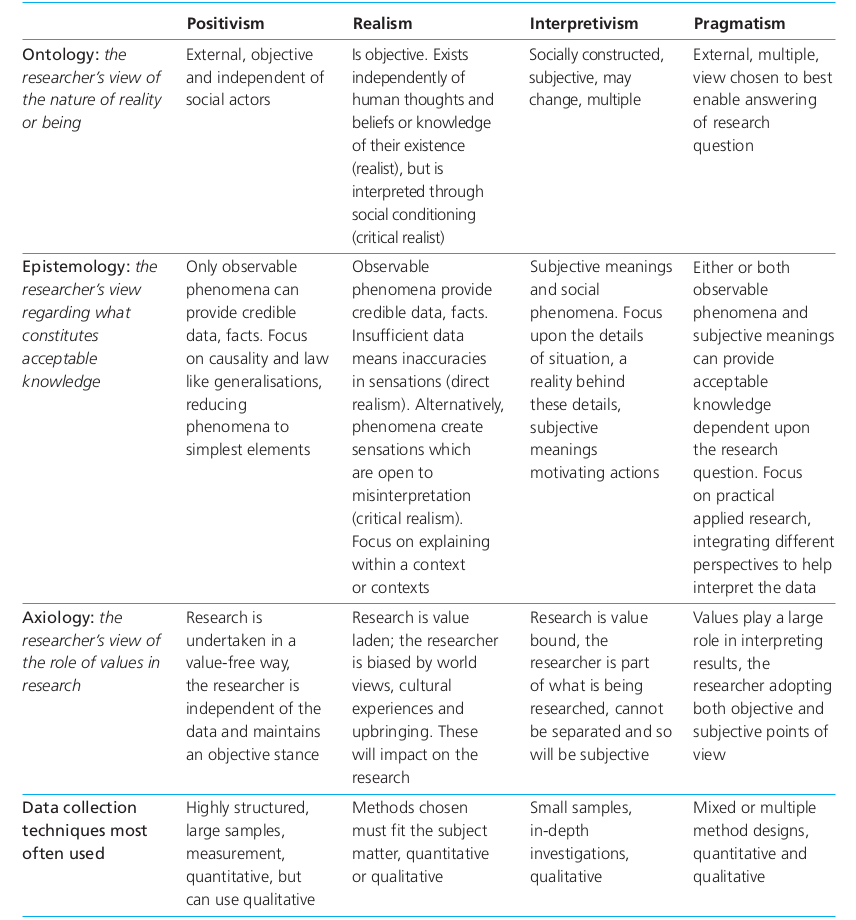
\includegraphics[width=1\linewidth]{img/comparison of research philosophies.png}
    \caption{Comparison of four research philosophies in management research}
    \label{fig:enter-label}
\end{figure}
\par{If the above figure is studied, a separation can be made regarding which research philosophy will be appropriate for the current research study. Positivism immediately stands out because of what its epistemology holds to be true, which is that the only reliable source of information that can be drawn upon is observable phenomena. This suits the current study very well as it will be dealing with a case study to implement a system and the conclusions regarding the success of the development project will be drawn from the success of created artefact or information system. The only other philosophy that has an epistemology aligned to the needs of the research project is realism, as it also views observable phenomena as credible sources of fact, although it opposes a direct reliance on observable phenomena as it believes they can be interpreted incorrectly or with a biased view. Interpretivism and pragmatism regard subjective meaning and social phenomena as the critical source of acceptable knowledge, which does not suit the circumstances of the research project. Therefore, interpretivism and pragmatism are ruled out as options for the chosen research philosophy for this project. }
\par{The remaining two options for viable research philosophies must be compared further to find a suitable methodology for the research project. Within the positivistic approach, the research is taken from a third party point of view to remain objective and reliant on the conclusions drawn from the outcome of the research project, while realism ascertains that the researcher is biased by world views and experiences and that this factors will have an impact on the research. As one of the critical purposes of this research project is to create a replicable methodology for how students can consistently build industry level software solutions, it is of the utmost importance that the researcher remain unbiased and objective. Therefore, according to the comparison of epistemology and axiology between positivism and realism, positivism is chosen as the preferred research philosophy for this project. }
\par{The next section encompasses the following stage within the modified research onion \citep{mardiana2020modifying}, the research approach. This section will be the entry point into the second layer of the research onion.}

\section{Research Approach}
\par{Research approaches make up the second layer of the Research Onion. A research strategy aids in the structure of a study by offering direction in determining the theory that the investigation seeks to advance \citep{saunders2009research}. There are three approaches that are offered by the the modified research, namely deduction, abduction, and induction. These three approaches are each investigated in more depth in the subsections that follow. Once they have been reviewed, a conclusion will be made on which option will be taken forward as the approach for this research project.}
\subsection{Deduction}
\par{In the deductive method, a hypothesis is generated alongside an established theory in order to test the theory \citep{saunders2009research}. When assessing qualitative data, the deductive and inductive approaches offer a thorough method. To make sense of the entire collection of data and comprehend what is taking place, this procedure entails fully immersing oneself in the reading and consumption of the material \citep{azungah2018qualitative}. Deductive qualitative research is distinct from other qualitative methodologies since it utilises conceptual premises generated from the review of literature as its starting point and employs them to the gathering and examination of data\citep{pearse2019illustration}.}
\par{Despite decades of exponential increases in computing capacity, the foundational ideas of the theories of computation still hold true. Thus, the importance of deductive research methods as a source of specific program knowledge has been established over time \citep{eden2007three}. \cite{knuth1968semantics} provides the following justification for his definition of computer science as a sub field of mathematics:}
\begin{quote}
"Like mathematics, computer science will be somewhat different from other sciences in that it deals with man-made laws, which can be [deductively] proved, instead of natural laws which are never known with certainty"
\end{quote}
\par{If the advice of \cite{knuth1968semantics} is taken into consideration alongside the fact that the current research field is computer science, the deductive approach could be very promising to achieving successful results in this project. The next subsection will outline abduction and the potential it holds for being the chosen research approach.}
\subsection{Abduction}
\par{When abduction was first used in 1597 by Julius Pacius to translate the Aristotelian apagoge, it went largely unrecognised for nearly three centuries. The term was initially used by C. S. Peirce \citep{smyth1999peirce}, who stated that it would represent the only fully knowledge-extending method of interpreting that would be categorically different from the two typical forms of logical conclusion, namely deduction and induction. In several artificial intelligence domains, including diagnosis, natural language comprehension, default reasoning, database updates, planning, and high-level vision, this type of abduction has become a common reasoning method.}
\par{Determining the most plausible explanation for a given collection of data is a challenge that can be classified as abduction \citep{josephson1987mechanism}. Abduction is applicable to many different types of reasoning exercises \citep{charniak1985introduction}. For instance, the final diagnosis in medicine clarifies the patient's symptoms and indicators \citep{pople1973mechanization,reggia1983diagnostic}. According to natural language comprehension, a sentence's intended meaning reveals why it was said \citep{hobbs1993interpretation}. Acceptance of a hypothesis in the establishment of scientific theory depends on how well it explains the data. In abductive reasoning, assumption A is accepted if it implies some observation 0 and aligns with preexisting beliefs \citep{lewis1982role}.}
\par{Abduction has become a common reasoning method in various artificial intelligence domains, including diagnosis, natural language comprehension, and planning. In the context of this master's thesis in computer science, abduction offers a systematic approach to evaluating student developers' capabilities and comparing their processes with industry standards, thereby aiding in the creation of an industry-standard ERP system for TaskFlow. Through its emphasis on determining the most plausible explanation for a given collection of data, abduction provides a valuable framework for ensuring the feasibility and success of the research project. As the project progresses, abduction will serve as a guiding principle for identifying and addressing challenges, iteratively improving the system, and ultimately contributing to the advancement of systems development methodologies within both academic and industrial settings.}
\subsection{Induction}
\par{Induction is widely used in the field of computer science (CS). Data structures, philosophy of computing \citep{lynch1996distributed,hopcroft2001introduction,barwise1998computers}, programming languages \citep{pierce2002types}, program efficiency-time complexity \citep{cormen2022introduction}, and algorithm correctness \citep{cormen2022introduction,lynch1996distributed,page2003software,weiss1998data} are only a few of the computer science fields that depend on it. Furthermore, induction can be employed as a teaching strategy to improve students' understanding and performance with CS concepts such as algorithm design, recursion, and programming languages \citep{manber1989introduction,wu1998conceptual}.  According to \cite{bruce2003math}, }
\begin{quote}
        "Programmers with a good understanding of mathematical induction find it much easier to write and, even more importantly, provide convincing arguments for the correctness of recursive algorithms."
\end{quote}
\par{However, research has shown that, even after receiving repeated training in several courses within their curriculum, students typically struggle to comprehend and execute proofs via induction \citep{lowenthal1992mathematical,movshovitz1993mathematical,baker1995characterizing,dubinsky1989teaching}. Even after receiving repeated teaching in several courses within their curriculum, it has been reported in the literature that students generally struggle to comprehend and execute proofs by induction \citep{polycarpou2008conceptual}.}
\par{In conclusion, induction serves as a foundational pillar within the field of computer science, playing a vital role across various domains Its significance extends beyond theoretical frameworks, as it also serves as a pedagogical tool to enhance students' understanding and proficiency in fundamental CS concepts. Despite its ubiquity and importance, empirical evidence suggests persistent challenges among students in grasping and applying inductive reasoning. Addressing these challenges requires a nuanced approach that combines theoretical instruction with practical application, leveraging insights from cognitive science and educational psychology to scaffold students' learning experiences effectively. By acknowledging the complexities inherent in mastering induction, educators and researchers can develop tailored interventions aimed at fostering deeper comprehension and proficiency in this essential aspect of computer science education that could lead to a successful outcome within this research project.}
\par{The research approach that is made use of within this research paper is deduction as it holds that with this approach a researcher begins with a hypothesis and then aims to acquire evidence to prove it, support it, or outrightly refute it. This approach is used by researchers when they want to test an existing hypothesis rigorously. Therefore, it is the most suited to what is being tested in this research project and will further be used as the research approach in this project aiming to make use of the assumption that students can build an ERP system of industry standards and put it to the test. The next section regards the third layer of the modified research onion called the research strategy, where the methods of data acquisition are investigated and the chosen method is then selected.}


\section{Research Strategy}


\section{Research Methodologies}
%What is a research methodology and what is its purpose? WRITE INTRODUCTION
\subsection{Design Science}
\par{The Design Science Research Methodology, or DSRM, was developed by \cite{peffers2007design} with three goals in keeping in mind: "(1) offer a nominal procedure for carrying out DS study, (2) expand on earlier research on DS in IS and related fields, and (3) offer scholars a conceptual model for a framework for the results of research.” The Design Science Research (DSR) paradigm is based on the artificial sciences and engineering. In essence, it is a paradigm for solving problems. DSR creates new artefacts in an attempt to advance human understanding \citep{hevner2010design}. In the past few years, a number of researchers have successfully brought design research into the realm of information science (IS) studies, such as \cite{hevner2004design} and \cite{walls1992building}. They are also effective in making design a major part of research and proving the value and legitimacy of design science (DS) as an IS research paradigm. In the fifteen years or more that have elapsed since those first articles, very little DS research has been successfully published in the IS field, despite these effective breaches \citep{peffers2007design} outlines a process that encompasses six activities that make up the DSR methodology and are arranged in a certain sequence that dictates the order of progression for research based on this methodology. The table below outlines these activities.:}
\clearpage
\begin{figure}[h!]
    \centering
    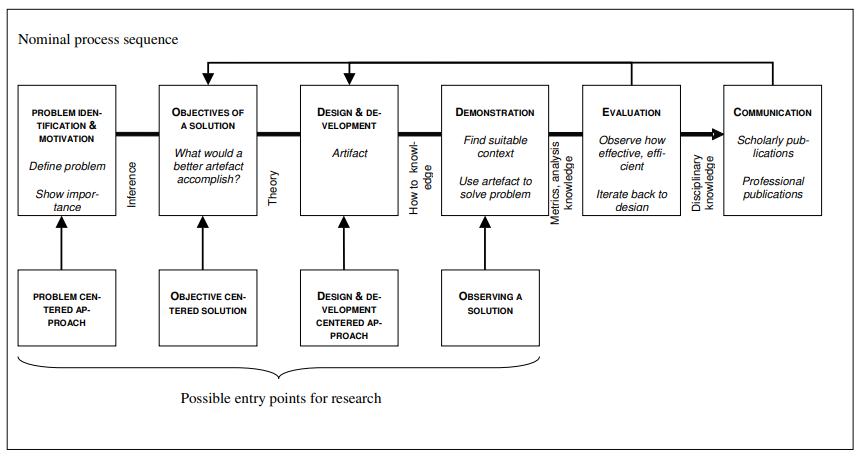
\includegraphics[width=1\linewidth]{img/Design science research process (DSRP) model.png}
    \caption{Design science research process (DSRP) model}
    \label{fig:enter-label}
\end{figure}
\par{The DSR methodology will be used to conduct the research project, thus each step outlined by \cite{peffers2007design} is investigated in broader context to better understand accurate execution and use of the research methodology.}
\par{\begin{enumerate}
        \item Problem Identification and Motivation
\par{Before coming up with viable solutions, designers work with vague problems that need more investigation (\citealt{buchanan1992wicked, rittel1973dilemmas}). Prescriptive engineering design procedures frequently place a strong emphasis on characterising an issue as the first step. Problem  is the driving force behind these problem-first approaches, which use design to find a solution \citep{dewey2022we}. There for it is of the utmost importance to correctly identify and define the problems and motivation within this research study.}
\par{The purpose of this first activity within the research methodology is of utmost importance as it designates the entry point to the entirety of what will be done within this research. \cite{peffers2007design} specifies what has to be done to properly identify the problem and motivation related to the study. The research problem has to be specified and an explanation to why a solution is valuable must be provided. It could be helpful to conceptually atomize the problem so that the solution can adequately represent the complexity of the problem, as the problem definition will be utilised to create an effective artifactual solution. Two goals are achieved when a solution is justified: first, it encourages the researcher and the research's audience to pursue the answer and accept the findings; second, it clarifies the logic behind the researcher's comprehension of the issue. Knowledge of the problem's current condition and the significance of its solution are among the resources needed for this task.}
        \item Objectives of the solution
\par{Determine a solution's goals based on the definition of the problem. The goals can be qualitative, such as when a new artefact is anticipated to enable answers to issues not previously addressed, or quantitative, such as terms in which a desirable solution would be preferable to current ones. The goals ought to be as follows: logically inferred from the problem description. Information about the current state of issues, existing solutions, and their efficacy, if any, are among the resources needed for this.}
        \item Design and Development
\par{}
        \item Demonstration
        \item Evaluation
        \item Communication
\end{enumerate}}
\subsection{Action Design Research}
\subsection{Action Research}
\subsection{Conclusion}


\section{Research Design}
A researcher's detailed approach for addressing his or her research question(s) is known as the research design \citep{mardiana2020modifying}.
\subsection{Data Collection}
\subsection{Ethical Considerations}


\section{Conclusion}
